% Neural network diagram
% Made with Xematics. Positions are in px (1 px = 0.75 pt), as in the SVG export.
\documentclass[tikz, border=4pt]{standalone}
\definecolor{xm1}{HTML}{FFFFFF}
\definecolor{xm2}{HTML}{6B7280}
\definecolor{xm3}{HTML}{D4E8F5}
\definecolor{xm4}{HTML}{0072B2}
\definecolor{xm5}{HTML}{1F2937}
\definecolor{xm6}{HTML}{4B5563}
\definecolor{xm7}{HTML}{F1F2F4}
\definecolor{xm8}{HTML}{FBE8C4}
\definecolor{xm9}{HTML}{B97800}
\begin{document}
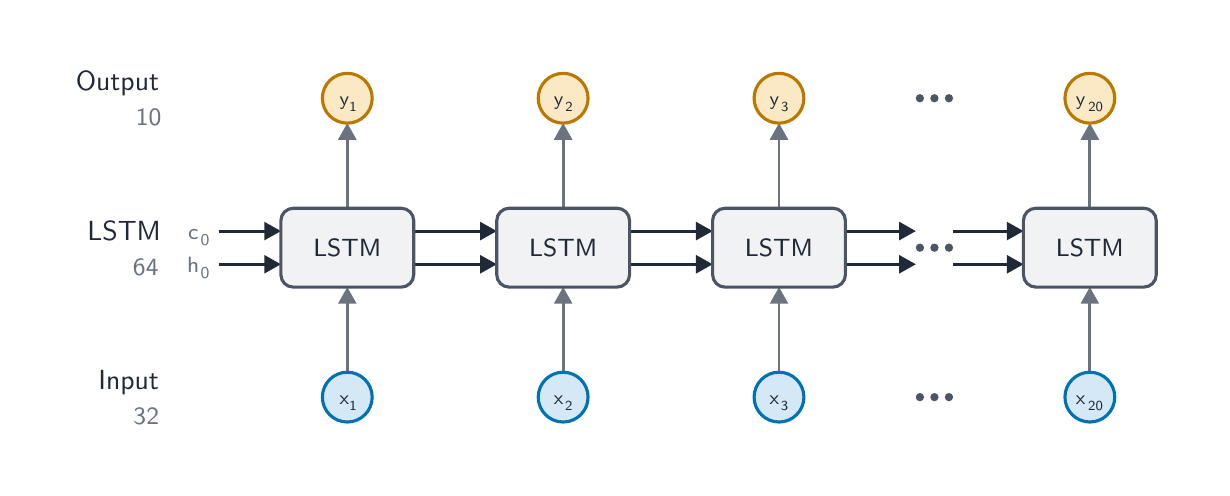
\begin{tikzpicture}[x=0.75pt, y=-0.75pt]
  \tikzset{
    xm arrow d6rgep/.style={draw=xm2, line width=1.05pt},
    xm arrow 14mtdps/.style={fill=xm2, line join=round},
    xm node 1gy69v8/.style={fill=xm3, draw=xm4, line width=1.13pt},
    xm text xm5/.style={text=xm5, inner sep=0},
    xm circle 1myn5on/.style={fill=xm6},
    xm state 1rxny0e/.style={draw=xm5, line width=1.05pt},
    xm state 1q719u5/.style={fill=xm5, line join=round},
    xm text xm2/.style={text=xm2, inner sep=0},
    xm box 100m3ez/.style={fill=xm7, draw=xm6, line width=1.13pt, rounded corners=4.5pt},
    xm node k2udt6/.style={fill=xm8, draw=xm9, line width=1.13pt},
  }
  \fill[xm1] (0,0) rectangle (565.75,212);
  % Diagram
  \path[xm arrow d6rgep] (153.99,166) -- (153.99,132);
  \path[xm arrow 14mtdps] (153.99,125) -- (158.49,133) -- (149.49,133) -- cycle;
  \path[xm arrow d6rgep] (257.99,166) -- (257.99,132);
  \path[xm arrow 14mtdps] (257.99,125) -- (262.49,133) -- (253.49,133) -- cycle;
  \path[xm arrow d6rgep] (361.99,166) -- (361.99,132);
  \path[xm arrow 14mtdps] (361.99,125) -- (366.49,133) -- (357.49,133) -- cycle;
  \path[xm arrow d6rgep] (511.75,166) -- (511.75,132);
  \path[xm arrow 14mtdps] (511.75,125) -- (516.25,133) -- (507.25,133) -- cycle;
  \path[xm arrow d6rgep] (153.99,87) -- (153.99,53);
  \path[xm arrow 14mtdps] (153.99,46) -- (158.49,54) -- (149.49,54) -- cycle;
  \path[xm arrow d6rgep] (257.99,87) -- (257.99,53);
  \path[xm arrow 14mtdps] (257.99,46) -- (262.49,54) -- (253.49,54) -- cycle;
  \path[xm arrow d6rgep] (361.99,87) -- (361.99,53);
  \path[xm arrow 14mtdps] (361.99,46) -- (366.49,54) -- (357.49,54) -- cycle;
  \path[xm arrow d6rgep] (511.75,87) -- (511.75,53);
  \path[xm arrow 14mtdps] (511.75,46) -- (516.25,54) -- (507.25,54) -- cycle;
  \path[xm node 1gy69v8] (153.99,178) circle[radius=12];
  \node[xm text xm5, font=\sffamily\fontsize{7.5}{9}\selectfont, anchor=base] at (152.53,181.64) {x};
  \node[xm text xm5, font=\sffamily\fontsize{5.4}{6.48}\selectfont, anchor=base] at (156.72,184.44) {1};
  \path[xm node 1gy69v8] (257.99,178) circle[radius=12];
  \node[xm text xm5, font=\sffamily\fontsize{7.5}{9}\selectfont, anchor=base] at (255.8,181.64) {x};
  \node[xm text xm5, font=\sffamily\fontsize{5.4}{6.48}\selectfont, anchor=base] at (260.72,184.44) {2};
  \path[xm node 1gy69v8] (361.99,178) circle[radius=12];
  \node[xm text xm5, font=\sffamily\fontsize{7.5}{9}\selectfont, anchor=base] at (359.77,181.64) {x};
  \node[xm text xm5, font=\sffamily\fontsize{5.4}{6.48}\selectfont, anchor=base] at (364.72,184.44) {3};
  \path[xm circle 1myn5on] (429.87,178) circle[radius=2];
  \path[xm circle 1myn5on] (436.87,178) circle[radius=2];
  \path[xm circle 1myn5on] (443.87,178) circle[radius=2];
  \path[xm node 1gy69v8] (511.75,178) circle[radius=12];
  \node[xm text xm5, font=\sffamily\fontsize{7.5}{9}\selectfont, anchor=base] at (507.29,181.64) {x};
  \node[xm text xm5, font=\sffamily\fontsize{5.4}{6.48}\selectfont, anchor=base] at (514.48,184.44) {20};
  \path[xm state 1rxny0e] (185.99,98) -- (218.99,98);
  \path[xm state 1q719u5] (225.99,98) -- (217.99,102.5) -- (217.99,93.5) -- cycle;
  \path[xm state 1rxny0e] (185.99,114) -- (218.99,114);
  \path[xm state 1q719u5] (225.99,114) -- (217.99,118.5) -- (217.99,109.5) -- cycle;
  \path[xm state 1rxny0e] (289.99,98) -- (322.99,98);
  \path[xm state 1q719u5] (329.99,98) -- (321.99,102.5) -- (321.99,93.5) -- cycle;
  \path[xm state 1rxny0e] (289.99,114) -- (322.99,114);
  \path[xm state 1q719u5] (329.99,114) -- (321.99,118.5) -- (321.99,109.5) -- cycle;
  \path[xm state 1rxny0e] (393.99,98) -- (420.87,98);
  \path[xm state 1q719u5] (427.87,98) -- (419.87,102.5) -- (419.87,93.5) -- cycle;
  \path[xm state 1rxny0e] (393.99,114) -- (420.87,114);
  \path[xm state 1q719u5] (427.87,114) -- (419.87,118.5) -- (419.87,109.5) -- cycle;
  \path[xm state 1rxny0e] (445.87,98) -- (472.75,98);
  \path[xm state 1q719u5] (479.75,98) -- (471.75,102.5) -- (471.75,93.5) -- cycle;
  \path[xm state 1rxny0e] (445.87,114) -- (472.75,114);
  \path[xm state 1q719u5] (479.75,114) -- (471.75,118.5) -- (471.75,109.5) -- cycle;
  \path[xm state 1rxny0e] (91.99,98) -- (114.99,98);
  \path[xm state 1q719u5] (121.99,98) -- (113.99,102.5) -- (113.99,93.5) -- cycle;
  \node[xm text xm2, font=\sffamily\fontsize{8.25}{9.9}\selectfont, anchor=base] at (79.85,102) {c};
  \node[xm text xm2, font=\sffamily\fontsize{5.94}{7.13}\selectfont, anchor=base] at (85.49,105.08) {0};
  \path[xm state 1rxny0e] (91.99,114) -- (114.99,114);
  \path[xm state 1q719u5] (121.99,114) -- (113.99,118.5) -- (113.99,109.5) -- cycle;
  \node[xm text xm2, font=\sffamily\fontsize{8.25}{9.9}\selectfont, anchor=base] at (79.74,118) {h};
  \node[xm text xm2, font=\sffamily\fontsize{5.94}{7.13}\selectfont, anchor=base] at (85.49,121.08) {0};
  \path[xm box 100m3ez] (121.99,87) rectangle ++(64,38);
  \node[xm text xm5, font=\sffamily\fontsize{9}{10.8}\selectfont, anchor=base] at (153.99,110.37) {LSTM};
  \path[xm box 100m3ez] (225.99,87) rectangle ++(64,38);
  \node[xm text xm5, font=\sffamily\fontsize{9}{10.8}\selectfont, anchor=base] at (257.99,110.37) {LSTM};
  \path[xm box 100m3ez] (329.99,87) rectangle ++(64,38);
  \node[xm text xm5, font=\sffamily\fontsize{9}{10.8}\selectfont, anchor=base] at (361.99,110.37) {LSTM};
  \path[xm circle 1myn5on] (429.87,106) circle[radius=2];
  \path[xm circle 1myn5on] (436.87,106) circle[radius=2];
  \path[xm circle 1myn5on] (443.87,106) circle[radius=2];
  \path[xm box 100m3ez] (479.75,87) rectangle ++(64,38);
  \node[xm text xm5, font=\sffamily\fontsize{9}{10.8}\selectfont, anchor=base] at (511.75,110.37) {LSTM};
  \path[xm node k2udt6] (153.99,34) circle[radius=12];
  \node[xm text xm5, font=\sffamily\fontsize{7.5}{9}\selectfont, anchor=base] at (152.53,37.64) {y};
  \node[xm text xm5, font=\sffamily\fontsize{5.4}{6.48}\selectfont, anchor=base] at (156.8,40.44) {1};
  \path[xm node k2udt6] (257.99,34) circle[radius=12];
  \node[xm text xm5, font=\sffamily\fontsize{7.5}{9}\selectfont, anchor=base] at (255.8,37.64) {y};
  \node[xm text xm5, font=\sffamily\fontsize{5.4}{6.48}\selectfont, anchor=base] at (260.8,40.44) {2};
  \path[xm node k2udt6] (361.99,34) circle[radius=12];
  \node[xm text xm5, font=\sffamily\fontsize{7.5}{9}\selectfont, anchor=base] at (359.77,37.64) {y};
  \node[xm text xm5, font=\sffamily\fontsize{5.4}{6.48}\selectfont, anchor=base] at (364.8,40.44) {3};
  \path[xm circle 1myn5on] (429.87,34) circle[radius=2];
  \path[xm circle 1myn5on] (436.87,34) circle[radius=2];
  \path[xm circle 1myn5on] (443.87,34) circle[radius=2];
  \path[xm node k2udt6] (511.75,34) circle[radius=12];
  \node[xm text xm5, font=\sffamily\fontsize{7.5}{9}\selectfont, anchor=base] at (507.29,37.64) {y};
  \node[xm text xm5, font=\sffamily\fontsize{5.4}{6.48}\selectfont, anchor=base] at (514.56,40.44) {20};
  \node[xm text xm5, font=\sffamily\fontsize{9.75}{11.7}\selectfont, anchor=base] at (48.67,174.47) {Input};
  \node[xm text xm2, font=\sffamily\fontsize{9}{10.8}\selectfont, anchor=base] at (57.13,191.23) {32};
  \node[xm text xm5, font=\sffamily\fontsize{9.75}{11.7}\selectfont, anchor=base] at (46.48,102.47) {LSTM};
  \node[xm text xm2, font=\sffamily\fontsize{9}{10.8}\selectfont, anchor=base] at (56.89,119.23) {64};
  \node[xm text xm5, font=\sffamily\fontsize{9.75}{11.7}\selectfont, anchor=base] at (43.25,30.47) {Output};
  \node[xm text xm2, font=\sffamily\fontsize{9}{10.8}\selectfont, anchor=base] at (58.27,47.23) {10};
\end{tikzpicture}
\end{document}
